
The ideas reflected in the previous chapters were implemented into a software platform called Braviz. This software is licensed under a LGPL license and its source code and documentation can be found online at http://diego0020.github.io/braviz . As suggested by user centered design, the software was the result of several iterations. The architecture of the software reflects the model described in chapter \ref{chap_model}. Details of these aspects will be given in the following. Finally we will describe some of the more technical details of the software.

\section{Iterations}

The development of the platform went trough several prototypes that were tested with target users. From each prototype several lessons were learned, both from the technical point and from the users feedback. Each iteration brings new ideas and challenges to the project. As the process goes on prototypes become more sophisticated. At the start changes occur very fast, while at the process goes on changes are smaller and take longer. The whole process can be seen as a spiral (see figure \ref{intro_spiral}). This section will provide an overview of each of the iterations up to the current point, and show the more significant insights and changes from each of them. Notice that the process has not stopped, and we expect the platform to continue evolving. Chapter \ref{chap_conclusions} will provide details of the plans for future iterations.

\subsection{Previous Work}

\begin{figure}
\centering
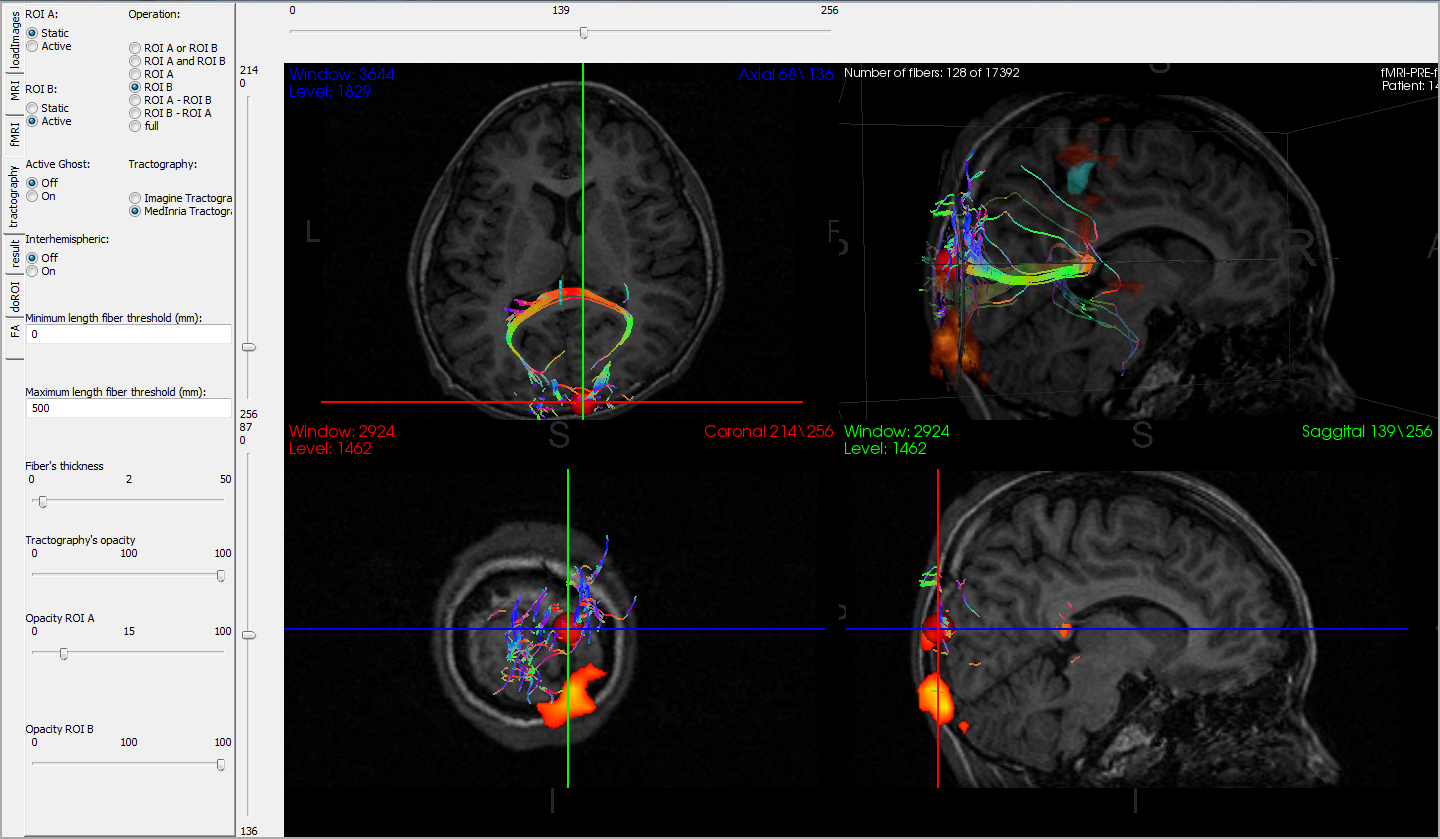
\includegraphics[width=0.9\textwidth]{historic/kab_figura1.png} 
\caption{\label{fig_kab}The main interface of KAB}
\end{figure}

The first prototype built by our group was called KAB \autocite{castro_kab:_2012}. This tool was built to analyze data from the KMC pilot study \autocite{schneider_cerebral_2012}. This software integrated data from Diffusion MRI, Functional MRI and structural MRI. The main interface of the tool is shown in figure \ref{fig_kab}. Data was pre-processed using FSL \autocite{jenkinson_fsl_2012} for skull removal and FMRI modeling, and Medinria \autocite{toussaint_medinria} for diffusion data. Registration between diffusion and structural spaces was done on-line using the tool itself. The most important features of the software were:

\begin{itemize}
\item Visualizing structural MRI, fMRI and tractography on the same space
\item Selection of bundles in a full tractography
\begin{itemize}
\item Using two spherical regions of interests located manually
\item Using conical regions of interests, representing the spread of TMS magnetic pulses
\item Using areas where fMRI statistics were above a threshold
\item Using hand-drawn regions
\end{itemize}
\item Generating statistics from selected bundles
\item Automatic generation of reports
\end{itemize}

Integrating information from different sources was the major contribution of the tool. Traditionally each type of data was analyzed on its own, using dedicated tools, and integrating information in this way was beyond brain experts. This tool was implemented based on the BBTK framework \autocite{} developed by Creatis.



- background
-- kab

\subsection{First prototypes}
-- titanic

\subsection{Braviz, First Version}
- Braviz/tk
-- sample applications

\subsection{Braviz, Second Version}
- Braviz Qt
-- sample applications

\subsection{Braviz, Third Version}


Iterations
-------------

- Feedback
- changes
- evidence of user centered design








\section{Architecture}

From model to implementation
-----------------------------

- architecture
- common platform
- skeleton of a application
- database


\section{Technical Details}

Technical details
------------------

- organization
- libraries
- messaging protocol
- data input/output
- transformations
- coordinate systems



